9 Cross Platform Mobile Frameworks were identified and compared. The 9 Frameworks were  found using the online Mobile Frameworks Comparison Chart. The target platforms where Android and iOS. The hardware features selected were Camera, Capture, Connection, File and Storage. In addition the framework should include UI Widgets and a free License. The following 9 frameworks were listed:

\begin{itemize}[label={}]
\item \textbf{AppGyver:} AppGyver is a hybrid solution based on Cordova/Phonegap. Cordova/Phonegap apps are programmed in javascript, using standard html/css for the interface, and wrapped in an application that is little more that a full screen web browser. Native functionality is made available through plugins. The AppGyver Supersonic device API does not allow a camera preview to be integrated into the UI or the app, this must be implemented using a 3rd party cordova plugin. The AppGyver Supersonic UI can be used to implement the UI Components of the app, or another UI Framework such as ionic could be integrated. In fact the only difference from AppGyver and ionic is that many AppGyver feature utilises an online developer environment which is a commercial service.

\item \textbf{Application Craft:} Like AppGyver, Application Craft is a based on Cordova/Phonegap. But the developer environment and deployment process is totally bound to the commercial online service. It is not clear from the developer documentation whether the applications are extendable with 3rd party plugins.

\item \textbf{Corona:} Cross-platform native solution, targeted toward game development. C++ and Lua are used for programming. The UI features are game oriented and do not offer many advantages for general mobile apps development.

\item \textbf{Framework7:} This is a professional looking cordova based solution. The UI features are excellent. Native functionality is extendable through 3rd party cordova plugins. Unfortunately Android is only partially supported.

\item \textbf{Gideros:} Gideros is a cross platform native solution that uses Lua for programming targeted toward game development. The feature set is similar to Corona. So are the limitations. The UI is not appropriate to general app development. The developer documentation is not clear regarding camera integration.

\item \textbf{ionic:} ionic is a mature UI framework built on Cordova/Phonegap. ionic is implemented using angular.js and offers a rich set of template directives which can be used to customise the user interface easily. Two-way data binding between logic controllers and view templates is also enabled through angular. The ionic developer also provides an online service that assists in development and deployment. Use of the service is completely optional though.

\item \textbf{Kivy:} Kivy is a python based framework that is compiled to native code. Unfortunately the UI components are not targeted toward general app development and are more game oriented.

\item \textbf{The-M-Project:} This is a hybrid cross platform framework that uses web technologies to provide the UI and logic. It leverages backbone.js to make UI development simpler. Its not clear in the documentation how camera access is enabled and to what extent. The framework does not appear to be based on Cordova/Phonegap so those 3rd part plugins might not be available.

\item \textbf{ViziApps:} Similar to AppGyper and Application Craft. This framework is Cordova/Phonegap based with a strong dependency on a commercial online development and deployment environment.

\end{itemize}

\subsection{Comparison}

\begin{itemize}[label={}]
\item \textbf{Cross-platform Support:} A minimum requirement for cross-platform support is that the framework allows the application to run on iOS and Android devices without any addition configuration.

Enabler of: OE-1, POR-1

\item \textbf{Integrated Camera Access:} The framework allows integrated access to the devices camera APIs. The MDApp will not simply pass the Smartphone User to the native camera mode. Instead the camera preview will be integrated in the MDApp user interface. If available on the native device the MDApp should also be able to set the focal range, center the focal point and be notified via a callback when the camera lens has focused so that it can notify the Smartphone User that it is ready to capture an image.

Enabler of: Image.Capture.Preview, Image.Capture.Trigger, SI-1.*

\item \textbf{Network Connectivity:} The framework allows the MDApp to connect via the internet to the online services required to perform the border analysis and risk assessment calculations. This includes uploading and downloading image files as well as posting and receiving data from an online API.

Enabler of: CI-1.*, CI-2.*, Border.Extract.Calculate, Risk.Assessment.Calculate

\item \textbf{Native File Access:} The framework allows the MDApp to save image files, captured by the camera or downloaded from the border extraction service, to be save internally on the native file system. Image files shall not only be saved in the devices image library but within the MDApp’s allocated storage. On iOS the image files shall be saved in the app internal “/Directory” folder. This directory is accessible and manageable by the user, it is also backed up via the iOS native backup strategies that the Smartphone User would be familiar with. On Android image files and data should be saved on the shared “External Storage” directory. This ensures that files and data are both accessible, backup-able, and persisted in the case of a software update.

Enabler of: SI-2, INT-1, INT-2, INT-3

\item \textbf{Native DB Storage:} Hybrid Apps generally live in a browser based context. Persistence of data is an issue therefore because in browsers data is generally transient. The framework chosen needs to offer a data solution either be tying in to native system data solutions ( CoreData on iOS for example ) or by providing an Sqlite file based solution.

Enabler of: INT-1, INT-2, INT-3, Metadata.Location.*, Metadata.Text.*, Archive.Save, Archive.Browse, Archive.Select.*

\item \textbf{UI Components:} The framework should include graphical user interface components and layout tools that assist in building a user interface that emulates the native look and feel of the platform. At the same time is should be consistent across all platforms. These are two conflicting requirements so some compromise is necessary to balance these aspects.

Enabler of: UI-5, UI-6, POR-1

\item \textbf{Unrestrictive License:} The framework should not be prohibitive with respect to intellectual property or financial cost. It should be open source with no restrictions on the distribution model for the app. The financial cost should be low, or free.

\item \textbf{Unrestrictive License:} Some frameworks are integrated with a service (usually commercial) that allow or restrict development to an online web based development environment. The chosen framework should not restrict development or deployment in any way.


\item \textbf{Advanced MVC Integration:} Does the framework offer tools that assist the developer to adhere to a modern MVC architecture? Integrated data-binding functionality, for example, allows data synchronisation between the view and controller.

Enabler of: TES-1, MOD-1

\end{itemize}

Figure \ref{fig:comp_fw} shows the comparison matrix applied to the 9 mobile cross-platform development framework.

\begin{figure}[H]
    \centering
    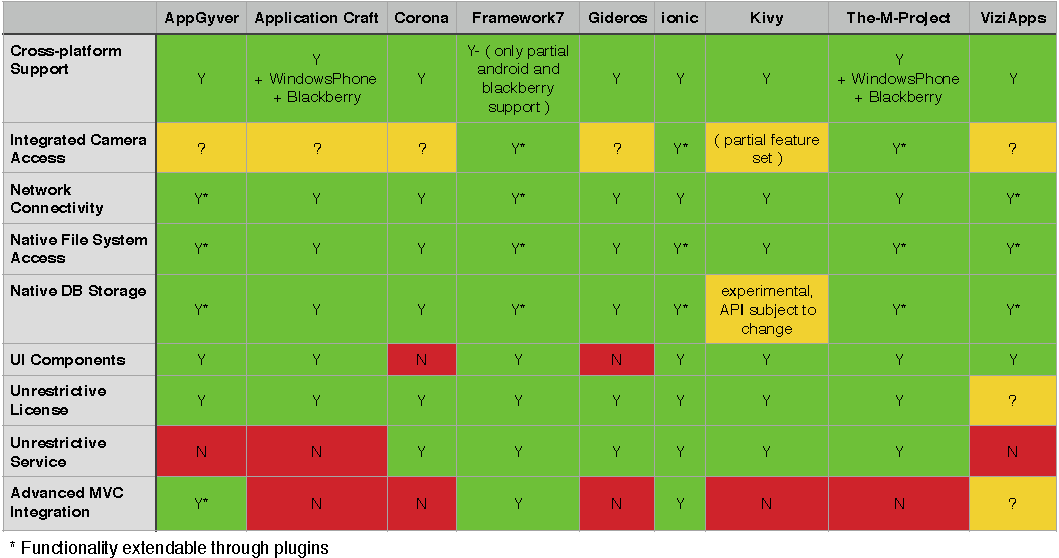
\includegraphics[width=\textwidth,keepaspectratio]{assets/architecture/framework_comparison.pdf}
    \caption{Mobile cross platform frameworks comparison}
    \label{fig:comp_fw}
\end{figure}

Framework7 and ionic score the best in the comparison chart above. Framework7 is a newer framework with no external dependencies. Ionic has been around longer and is basically a mobile UI framework that is built upon AngularJS, bringing with it all the features that make browser based development easier. Two-way data binding, tempting, and RESTful programming resources are some of the highlights of Angular. Because of these features and the widely available programming resources, references, and documentation ionic has been chosen as the framework to implement the MDApp.

